\documentclass[a4paper]{article}
\usepackage{amsmath, amsfonts, geometry, float, listings, enumerate, multicol}
\usepackage{multicol, float, colortbl}
\usepackage{lipsum}
\usepackage{tikz, titlesec, parskip}
\usepackage{tikz,pgfplots, circuitikz}
\usepackage{epsfig,graphicx,amsthm,amsmath}
\usepackage{wrapfig}
\usepackage{subfigure}
\usepackage{caption}
\usepackage{pythontex} 
\usepackage{matlab-prettifier}
\usepackage{tabularx}
\usepackage{media9}
\usepackage[utf8]{inputenc}
\usepackage{color}
\usepackage[symbol]{footmisc}
\usepackage{listings,lstautogobble}
\usepackage{lipsum}
\usepackage{parskip}
\usepackage{booktabs}
\usepackage{soul}
\usepackage[T1]{fontenc}
\usepackage{geometry}
\usepackage{titlesec}
\usepackage{booktabs}
\usepackage{multirow}
\usepackage{amssymb}

\usepackage{caption, enumitem}
\definecolor{forest}{RGB}{34,139,34}
\definecolor{codebg}{RGB}{30, 30, 46}
\definecolor{codefg}{RGB}{205, 214, 244}
\definecolor{codecomment}{RGB}{137, 180, 250}
\definecolor{codekeyword}{RGB}{203, 166, 247}
\definecolor{codestring}{RGB}{166, 227, 161}
\definecolor{codeerror}{RGB}{243, 139, 168}
\definecolor{sectionbg}{RGB}{30, 30, 46}
\definecolor{sectionfg}{RGB}{137, 180, 250}
\definecolor{tablehead}{RGB}{49, 50, 68}
\definecolor{tablerow}{RGB}{69, 71, 90}
\usetikzlibrary{arrows,calc,positioning}
\tikzset{
	block/.style = {draw, rectangle,
		minimum height=1cm,
		minimum width=2cm},
	input/.style = {coordinate,node distance=1cm},
	output/.style = {coordinate,node distance=4cm},
	arrow/.style={draw, -latex,node distance=2cm},
	pinstyle/.style = {pin edge={latex-, black,node distance=2cm}},
	sum/.style = {draw, circle, node distance=1cm},
}

\usepackage{relsize}
\usepackage[pagebackref=false,colorlinks,linkcolor=forest,urlcolor= blue,citecolor=blue]{hyperref}

\titlespacing{\section}{0pt}{10pt}{0pt}
\titlespacing{\subsection}{0pt}{10pt}{0pt}
\titlespacing{\subsubsection}{0pt}{10pt}{0pt}

\usetikzlibrary{calc,patterns,through}
\newcommand{\arcangle}{%
	\mathord{<\mspace{-9mu}\mathrel{)}\mspace{2mu}}%
}

\newcommand{\Cross}{$\mathbin{\tikz [x=1.4ex,y=1.4ex,line width=.2ex] \draw (0,0) -- (1,1) (0,1) -- (1,0);}$}%


\renewcommand{\baselinestretch}{1.2}
\geometry{
	a4paper,
	total={170mm,257mm},
	left=20mm,
	top=20mm,
}

\usepackage{hyperref}
\hypersetup{
	colorlinks=true,
	linkcolor=forest,
	filecolor=magenta,      
	urlcolor=cyan,
	pdftitle={Overleaf Example},
	pdfpagemode=FullScreen,
}

\usepackage{fancyhdr}
\pagestyle{fancy}
\fancyhf{}
\rhead{\textbf{ Farzan Aghaei }}
\lhead{\textbf{ Final Project }}
\lfoot{(\space\textbf{\thepage}\space)}
\rfoot{\textbf{Data Networks }}
\renewcommand{\headrulewidth}{1pt}
\renewcommand{\footrulewidth}{1pt}

\lstset{
	backgroundcolor=\color{codebg},
	basicstyle=\ttfamily\color{codefg}\footnotesize,
	commentstyle=\color{codecomment},
	keywordstyle=\color{codekeyword},
	stringstyle=\color{codestring},
	numbers=left,
	numberstyle=\tiny\color{gray},
	stepnumber=1,
	numbersep=5pt,
	frame=single,
	framerule=0pt,
	framesep=3pt,
	rulecolor=\color{codebg},
	breaklines=true,
	breakatwhitespace=true,
	tabsize=4,
	captionpos=b,
	showspaces=false,
	showstringspaces=false,
	showtabs=false,
	escapeinside={(*}{*)}
}

\begin{document}
	
	\begin{minipage}{0.65\textwidth}
		\begin{center}
			\normalsize
			‫		In the name of Allah\\
			\vspace{0.5cm}
			\huge
			\textbf{Data Networks} \\
			\vspace{0.2cm}
			\LARGE
			Prof. Mohammad Reza Pakravan \\
			\vspace{0.5cm}
			\Large
			Final Project\\
			\vspace{0.6cm}
			Farzan Aghaei 401101202
			\vspace{0.2cm}
		\end{center}
		\normalsize
	\end{minipage}
	\begin{minipage}{0.35\textwidth}
		\begin{flushleft}
			\centering
			
\includegraphics[width=0.7\textwidth]{Shariflogo.jpg}\\
			\large
			\vspace{0.4cm}
			Sharif University of Technology\\
			\vspace{0.2cm}
			Electrical Engineering Department\\
			\vspace{0.2cm}
		\end{flushleft}
	\end{minipage}
	
	\rule[0.1\baselineskip]{\textwidth}{1pt}

	\tableofcontents
	
	\pagebreak
	
	\section{Introduction}
	\label{sec:introduction}
	
	A proxy server acts as an intermediary between clients (web browsers) and destination servers. Instead of clients connecting directly to servers, they connect to the proxy server, which forwards requests and returns responses. This architecture provides several benefits:
	
	\begin{itemize}
		\item \textbf{Content Filtering}: Block access to specific URLs
		\item \textbf{Performance Improvement}: Cache frequently accessed resources
		\item \textbf{Traffic Monitoring}: Log and analyze network requests
		\item \textbf{Security}: Add an additional layer between clients and servers
	\end{itemize}
	
	In this project I implemented a comprehensive HTTP proxy server with the following features:
	
	\begin{itemize}
		\item Complete HTTP proxy functionality with TCP socket handling
		\item URL blocking with customizable lists
		\item Response caching for performance optimization
		\item Traceroute utility for network diagnostics
		\item Modern GUI for real-time monitoring
		\item Threaded architecture for concurrent request handling
		\item Status indicators and statistics
	\end{itemize}
	
	The proxy server was developed in Python using socket programming, threading, and Tkinter. The following sections provide a detailed explanation of both the core functionality and user interface implementation.
	
	\section{Core Functionality}
	\label{sec:core}
	
	The core functionality of the proxy server is implemented in a class named \texttt{HTTPProxyServer}. This class handles all network operations, request processing, and management features using socket and threading modules.
	
	The methods in this class are:
	\begin{itemize}
		\item log
		\item start
		\item stop
		\item accept\_connections
		\item parse\_request
		\item handle\_client
		\item is\_blocked
		\item load\_blocked\_urls
		\item clear\_blocked\_urls
		\item get\_cached\_url
		\item clear\_cache
		\item run\_traceroute
	\end{itemize}
	
	In the following parts of this section I will explain what each of these methods do and the functionality of the core.
	
	\pagebreak
	
	\subsection{Class Initialization}
	\vspace{0.5cm}
	\begin{lstlisting}[language=Python, caption=HTTPProxyServer Class Initialization]
class HTTPProxyServer:
	def __init__(self, port=8080):
		self.port = port  # Listening port for proxy
		self.running = False  # Server state flag
		self.server_socket = None  # Server socket
		self.cache = {}  # Cache storage
		self.blocked_urls = set()  # URLs to block
		self.lock = threading.Lock()  # Thread synchronization lock
		self.log_callback = None  # Logging callback function
		self.request_count = 0  # Total requests count
		self.blocked_count = 0  # Blocked requests count
		self.cache_hits = 0  # Cache hits count
	\end{lstlisting}
	
	The initialization method sets up the proxy's base components:
	
	\begin{itemize}
		\item \texttt{port}: The TCP port on which the proxy listens for client connections (default: 8080)
		\item \texttt{running}: Boolean flag indicating whether the server is currently active
		\item \texttt{server\_socket}: The main socket object that accepts incoming connections
		\item \texttt{cache}: Dictionary that stores cached responses with URLs as keys
		\item \texttt{blocked\_urls}: Set containing URLs that should be blocked
		\item \texttt{lock}: Threading lock to ensure thread-safe access to shared resources
		\item \texttt{log\_callback}: Function reference for logging messages to the GUI
		\item Statistics counters: Track request count, blocking activity, and cache performance
	\end{itemize}
	
	\subsection{Server Functionality Management}
	
	The server working cycle is controlled through the mentioned methods, which manage the server's operation.
	
	\subsubsection{start method}
	\vspace{0.5cm}
	\begin{lstlisting}[language=Python, caption=Server Start Method]
	def start(self):
		if self.running:
			return False
		self.running = True
		
		self.server_socket = socket.socket(socket.AF_INET, socket.SOCK_STREAM)
		self.server_socket.setsockopt(socket.SOL_SOCKET, socket.SO_REUSEADDR, 1)
		self.server_socket.bind(('127.0.0.1', self.port))
		self.server_socket.listen(8)
		
		self.log(f"Proxy server started on port {self.port}", "success")
		threading.Thread(target=self.accept_connections).start()
		return True
	\end{lstlisting}
	
	The \texttt{start()} method performs the following operations:
	
	\begin{itemize}
		\item Checks if the server is already running to prevent duplicate starts
		\item Creates a TCP socket using IPv4 addressing and stream-oriented protocol
		\item Sets socket option to allow address reuse for quick restarts
		\item Binds the socket to localhost (127.0.0.1) and the specified port
		\item Sets the socket to listening mode with a backlog of 8 pending connections
		\item Starts a thread running \texttt{accept\_connections()} to handle incoming connections
		\item Logs the start event
		\item Returns True on success and False on failure
	\end{itemize}
	
	\subsubsection{stop method}
	\vspace{0.5cm}
	\begin{lstlisting}[language=Python, caption=Server Stop Method]
	def stop(self):
		if not self.running:
			return
	
		self.running = False
		if self.server_socket:
			self.server_socket.close()
		self.log("Proxy server stopped")
	\end{lstlisting}
	
	The \texttt{stop()} method performs the following operations:
	
	\begin{itemize}
		\item Checks if the server is running to avoid unnecessary operations
		\item Updates the running state flag to False
		\item Closes the server socket to stop accepting new connections
		\item Logs the shutdown event
	\end{itemize}
	
	\subsubsection{accept\_connections method}
	\vspace{0.5cm}
	\begin{lstlisting}[language=Python, caption=Connection Acceptance Loop]
	def accept_connections(self):
		while self.running:
			try:
				client_socket, addr = self.server_socket.accept()
				self.request_count += 1
				threading.Thread(target=self.handle_client,
								 args=(client_socket, addr)).start()
			
			except OSError:
				break
	\end{lstlisting}
	
	The \texttt{accept\_connections()} method runs in a dedicated thread and performs:
	
	\begin{itemize}
		\item Continuous loop while the server is running
		\item Accepts incoming client connections using \texttt{accept()} function in socket
		\item Increments the total request counter
		\item Starts a new thread for each client connection to handle requests
		\item Catches \texttt{OSError} exceptions that occur when the socket is closed during shutdown
	\end{itemize}
	
	The new thread passes the requests to \texttt{handle\_client()} method.
	
	The \texttt{OSError} exception is added because the application kept giving an irrelevant OS error when the socket was closed, So I used try-except structure to break the loop when the error was generated (when the socket was closed).
	
	\pagebreak
	
	\subsubsection{parse\_request method}
	\vspace{0.5cm}
	\begin{lstlisting}[language=Python, caption=HTTP Request Parsing]
	def parse_request(self, request):
		lines = request.split('\r\n')
		method, url, http_version = lines[0].split()
		
		headers = {}
		for line in lines[1:]:
			if not line:
				break
			if ': ' in line:
				key, value = line.split(': ', 1)
				headers[key] = value
		
		return method, url, http_version, headers
	\end{lstlisting}
	
	The HTTP request and response structure is illustrated in the figure below.
	
	\begin{figure}[!h]
		\centering
		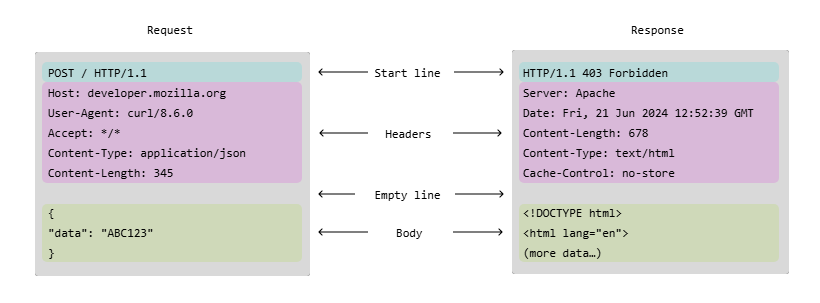
\includegraphics[width=\linewidth]{screenshot001}
		\caption{The structure of HTTP request and response messages}
		\label{fig:screenshot001}
	\end{figure}
	
	The request parser:
	
	\begin{itemize}
		\item Splits the request into individual lines
		\item Extracts the HTTP method, URL, and version from the request line (start line)
		\item Parses headers into key-value pairs (the header is kept in a dictionary variable)
		\item Handles header continuation and proper delimiter detection
		\item Returns method, url, http\_version and headers
	\end{itemize}
	
	Using this method I managed to break the requests into their components and separate them.
	
	\subsubsection{handle\_client method}
	\vspace{0.5cm}
	\begin{lstlisting}[language=Python, caption=Client Request Handling]
	def handle_client(self, client_socket, addr):
		try:
			request = client_socket.recv(1024).decode()
			if not request:
				return
			
			# Parse HTTP request
			method, url, http_version, headers = self.parse_request(request)
			
			# Extract host and path
			host = headers.get('Host', '')
			if not host:
				return
			
			self.log(f"Request #{self.request_count}: {method} {url} from {addr[0]}", "request")
			
			# Check if URL is blocked
			if self.is_blocked(url):
				self.blocked_count += 1
				self.log(f"Blocked URL: {url}", "blocked")
				response = (
				"HTTP/1.1 403 Forbidden\r\n"
				"Content-Type: text/html\r\n\r\n"
				"<html><body style='background: #1e1e2e; color: #cdd6f4; font-family: sans-serif; padding: 	40px; text-align: center;'>"
				"<h1 style='color: #f38ba8;'>403 Forbidden</h1>"
				"<p style='font-size: 1.2em;'>This URL has been blocked by the proxy server.</p>"
				"</body></html>"
				)
				client_socket.sendall(response.encode())
				return
			
			# Check cache
			cached_response = self.get_cached_url(url)
			if cached_response:
				self.cache_hits += 1
				self.log(f"Serving from cache: {url}", "cache")
				client_socket.sendall(cached_response)
				return
			
			# Forward request to destination server
			with socket.socket(socket.AF_INET, socket.SOCK_STREAM) as server_socket:
				server_socket.connect((host, 80))
				server_socket.sendall(request.encode())
				response = b""
				while True:
					response = server_socket.recv(32768)
					client_socket.sendall(response)
					break
			
			# Cache the response
			if method == "GET" and (response.startswith(b"HTTP/1.1 200") or response.startswith(b"HTTP/1.1 304")):
				if url not in self.cache:
					self.cache[url] = response
					self.log(f"Cached: {url}", "cache")
		
		except Exception as e:
			self.log(f"Error: {str(e)}", "error")
		
		finally:
			client_socket.close()
	\end{lstlisting}
	
	The request handling process performs the following operations:
	
	\begin{itemize}
		\item Receives and decodes the client request
		\item Parses the HTTP request into its components
		\item Checks for the existence of the Host header
		\item Logs the request details
		\item Checks if the URL is blocked and responds with 403 Forbidden if so
		\item Checks the cache for existing responses
		\item Forwards the request to the destination server
		\item Streams the response back to the client
		\item Caches successful GET responses
	\end{itemize}
	
	\subsubsection{url blocking methods}
	\vspace{0.5cm}
	\begin{lstlisting}[language=Python, caption=URL Blocking Implementation]
	def is_blocked(self, url):
		with self.lock:
			return any(blocked_url in url for blocked_url in self.blocked_urls)
	
	def load_blocked_urls(self, filename):
		with open(filename) as f:
			with self.lock:
				self.blocked_urls = {line.strip() for line in f if line.strip()}
		self.log(f"Loaded {len(self.blocked_urls)} blocked URLs", "success")
		return
	
	def clear_blocked_urls(self):
		with self.lock:
			self.blocked_urls.clear()
		self.log("Cleared blocked URLs")
	\end{lstlisting}
	
	The URL blocking system features:
	
	\begin{itemize}
		\item \texttt{is\_blocked()}: Checks if URL contains any blocked substring
		\item \texttt{load\_blocked\_urls()}: Loads URLs from a text file
		\item \texttt{clear\_blocked\_urls()}: Clears blocked URL list
		\item Thread-safe operations using locking
		\item Partial URL matching (block "example.com" blocks subdomains and paths)
	\end{itemize}
	
	\subsubsection{cache methods}
	\vspace{0.5cm}
	\begin{lstlisting}[language=Python, caption=Caching Implementation]
    def get_cached_url(self, url):
		with self.lock:
			return self.cache.get(url)
	
	def clear_cache(self):
		with self.lock:
			self.cache.clear()
		self.log("Cache cleared")

	\end{lstlisting}
	
	Caching mechanism:
	
	\begin{itemize}
		\item Dictionary-based storage with URL as key and response as value
		\item Thread-safe access using locking
		\item Only caches successful GET responses (HTTP 200 and HTTP 304)
		\item Cache persists until explicitly cleared
	\end{itemize}
	
	\subsubsection{run\_traceroute method}
	\vspace{0.5cm}
	\begin{lstlisting}[language=Python, caption=Traceroute Implementation]
	def run_traceroute(self, host):
		# Determine the correct command for the OS
		if platform.system().lower() == "windows":
			command = ['tracert', '-d', '-h', '5', host]
		else:
			command = ['traceroute', '-m', '5', host]
		
		result = subprocess.run(command, capture_output=True, text=True).stdout
		return result
	\end{lstlisting}
	
	Traceroute features:
	
	\begin{itemize}
		\item OS detection for command compatibility
		\item Runs the traceroute command using the subprocess module
		\item Captures the output streams
		\item Returns formatted output
	\end{itemize}
	
	\section{GUI Implementation}
	\label{sec:gui}
	
	The graphical user interface is implemented in the \texttt{ProxyGUI} class, providing visual control and monitoring for the proxy server. Built using Tkinter and ttk widgets, it features a modern dark theme with responsive components and real-time statistics.
	
	\subsection{Class Initialization}
	\vspace{0.5cm}
	\begin{lstlisting}[language=Python, caption=ProxyGUI Class Initialization]
class ProxyGUI:
	def __init__(self):
		self.proxy = ProxyServer()
		self.proxy.log_callback = self.log_message
		
		# Create main window
		self.root = tk.Tk()
		self.root.title("HTTP Proxy Server")
		self.root.geometry("960x640")
		self.root.configure(bg="#1e1e2e")
		self.root.minsize(900, 600)
		
		# Configure styling
		self.style = ttk.Style(self.root)
		self.style.theme_use("clam")
		self.configure_styles()
		
		# Create widgets
		self.create_widgets()
		
		# Set app icon
		self.set_icon()
		
		# Set initial status color to red (disconnected)
		self.update_status_color()
	\end{lstlisting}
	
	\pagebreak
	
	Key initialization elements:
	\begin{itemize}
		\item \texttt{proxy}: Instance of the core ProxyServer
		\item \texttt{log\_callback}: Connects core logging to GUI display
		\item Main window configuration: Dark theme (\#1e1e2e) with dimensions 960x640 and minimum size constraints 900x600
		\item Style Configuration: Uses 'clam' theme with custom dark mode adaptations
		\item Widget Creation: Creates the needed widgets
		\item App Icon: Sets up a custom icon for the application
		\item Initial Proxy Status Color: Sets the initial proxy status color to red (disconnected)
	\end{itemize}
	
	\subsection{Style Configuration}
	\vspace{0.5cm}
	\begin{lstlisting}[language=Python, caption=configure\_styles method]
	def configure_styles(self):
		# Configure colors
		bg_color = "#1e1e2e"
		fg_color = "#cdd6f4"
		
		self.style.configure(".", background=bg_color, foreground=fg_color,
							 font=("Inter", 10))
		self.style.configure("TFrame", background=bg_color)
		self.style.configure("TLabel", background=bg_color, foreground=fg_color)
		self.style.configure("TButton", background="#45475a", foreground=fg_color,
							 borderwidth=1, focuscolor="#89b4fa", padding=6)
		self.style.map("TButton", background=[("active", "#5c5e7e"), ("pressed", "#313244")],
					   foreground=[("active", fg_color)])
		self.style.configure("TEntry", fieldbackground="#313244", foreground=fg_color,
							 insertcolor=fg_color, padding=5)
		self.style.configure("TCombobox", fieldbackground="#313244", foreground=fg_color)
		self.style.configure("TNotebook", background=bg_color, borderwidth=0)
		self.style.configure("TNotebook.Tab", background="#313244", foreground=fg_color, 
							 padding=[10, 5], font=("Inter", 10, "bold"))
		self.style.map("TNotebook.Tab", background=[("selected", bg_color),
					   ("active", "#45475a")], foreground=[("selected", "#89b4fa")])
		self.style.configure("Vertical.TScrollbar", background="#45475a", arrowcolor=fg_color)
		
		# Configure tags for log text
		self.log_tags = {
			"info": {"foreground": "#89b4fa"},
			"error": {"foreground": "#f38ba8"},
			"success": {"foreground": "#a6e3a1"},
			"request": {"foreground": "#cba6f7"},
			"cache": {"foreground": "#f9e2af"},
			"blocked": {"foreground": "#f38ba8"},
			"system": {"foreground": "#a6e3a1"}
		}
	\end{lstlisting}
	
	The custom style configuration:
	\begin{itemize}
		\item Establishes consistent color scheme for dark mode UI
		\item Configures base styles for all widgets
		\item Defines color tags for log message categorization
		\item Ensures visual coherence across interface components
	\end{itemize}
	
	\pagebreak
	
	\subsection{Widget Creation}
	\vspace{0.5cm}
	\begin{lstlisting}[language=Python, caption=Main Widgets Construction]
	def create_widgets(self):
		# Create tabbed interface
		notebook = ttk.Notebook(self.root)
		
		# Control Panel Tab
		control_tab = ttk.Frame(notebook)
		notebook.add(control_tab, text="Control Panel")
		
		# Server Control Section
		control_frame = ttk.LabelFrame(control_tab, text="Server Management")
		control_frame.pack(fill=tk.X, padx=15, pady=15)
		
		# Port configuration
		ttk.Label(control_frame, text="Proxy Port:").grid(row=0, column=0)
		self.port_var = tk.StringVar(value="8080")
		port_entry = ttk.Entry(control_frame, textvariable=self.port_var, width=8)
		port_entry.grid(row=0, column=1)
		
		# Control buttons
		self.start_btn = ttk.Button(control_frame, text="Start", 
		command=self.start_proxy)
		self.start_btn.grid(row=0, column=2, padx=5)
		
		self.stop_btn = ttk.Button(control_frame, text="Stop", 
		command=self.stop_proxy, state=tk.DISABLED)
		self.stop_btn.grid(row=0, column=3, padx=5)
		
		# Statistics display
		stats_frame = ttk.Frame(control_frame)
		stats_frame.grid(row=0, column=4, sticky="e")
		ttk.Label(stats_frame, text="Requests:").pack(side=tk.LEFT)
		self.req_var = tk.StringVar(value="0")
		ttk.Label(stats_frame, textvariable=self.req_var).pack(side=tk.LEFT)
		
		# Activity Log Tab
		log_tab = ttk.Frame(notebook)
		notebook.add(log_tab, text="Activity Log")
		
		# Log display
		self.log_text = scrolledtext.ScrolledText(
		log_tab, bg="#313244", fg=fg_color, 
		font=("Consolas", 10), wrap=tk.WORD
		)
		self.log_text.pack(fill=tk.BOTH, expand=True)
		
		# Configure log colors
		for tag, style in self.log_tags.items():
		self.log_text.tag_config(tag, **style)
	\end{lstlisting}
	
	GUI component structure:
	\begin{itemize}
		\item Tabbed notebook interface for organized functionality (Control panel and Activity log)
		\item Control panel: Port configuration, command buttons, traceroute and statistics
		\item Real-time statistics: Total/Blocked/Cached request counters with live updating
		\item Activity log: Color-coded scrolling results and stats area
	\end{itemize}
	
	\subsection{App Icon}
	\vspace{0.5cm}
	\begin{lstlisting}[language=Python, caption=set\_icon method]
	def set_icon(self):
		myAppID = 'arbitrary string'
		ctypes.windll.shell32.SetCurrentProcessExplicitAppUserModelID(myAppID)
		self.root.iconbitmap("F:\\term6\data_network\project\\python\proxy.ico")
	\end{lstlisting}
	
	Using this method I managed to set a custom icon for my proxy app.
	
	\subsection{Status Color Update}
	\vspace{0.5cm}
	\begin{lstlisting}[language=Python, caption=update\_status\_color method]
	def update_status_color(self):
		if self.proxy.running:
			self.status_label.configure(foreground="#a6e3a1")  # Green when connected
		else:
			self.status_label.configure(foreground="#f38ba8")  # Red when disconnected
	\end{lstlisting}
	
	This method uses the running boolean element of the proxy server to update the color of the status label. The label will be green if connected and red if not.
	
	\subsection{Core Integration Methods}
	
	\subsubsection{Proxy Control Methods}
	\vspace{0.5cm}
	\begin{lstlisting}[language=Python, caption=Proxy Control Functions]
    def start_proxy(self):
		try:
			port = int(self.port_var.get())
			if not (1024 <= port <= 65535):
				raise ValueError("Port must be between 1024 and 65535")
		
			self.proxy.port = port
			if self.proxy.start():
				self.status_var.set(f"Status: Running on port {port}")
				self.start_button.config(state=tk.DISABLED)
				self.stop_button.config(state=tk.NORMAL)
				self.log(f"Proxy started on port {port}", "success")
				self.update_status_color()
			except Exception as e:
				self.log(f"Failed to start proxy: {str(e)}", "error")
				messagebox.showerror("Error", f"Failed to start proxy:\n{str(e)}")
		
		def stop_proxy(self):
			self.proxy.stop()
			self.status_var.set("Status: Not running")
			self.start_button.config(state=tk.NORMAL)
			self.stop_button.config(state=tk.DISABLED)
			self.log("Proxy server stopped")
			self.update_status_color()
	\end{lstlisting}
	
	Control flow features:
	\begin{itemize}
		\item Input validation for port number
		\item State management for control buttons
		\item Error handling while starting the proxy
		\item Updating the status color
		\item Logging the status changes
	\end{itemize}
	
	\subsubsection{Logging System}
	\vspace{0.5cm}
	\begin{lstlisting}[language=Python, caption=Logging Implementation]
	def log(self, message, tag="info"):
		self.log_text.config(state=tk.NORMAL)
		self.log_text.insert(tk.END, message + "\n", tag)
		self.log_text.config(state=tk.DISABLED)
		self.log_text.see(tk.END)
		
		# Update statistics
		self.request_count_var.set(str(self.proxy.request_count))
		self.blocked_count_var.set(str(self.proxy.blocked_count))
		self.cache_hits_var.set(str(self.proxy.cache_hits))
		
	def log_message(self, message, tag="info"):
		self.log(message, tag)
	\end{lstlisting}
	
	Logging system characteristics:
	\begin{itemize}
		\item Automatic scrolling to newest entries
		\item Color coding based on message type
		\item Real-time statistics updating
		\item State management for text widget
	\end{itemize}
	
	\subsubsection{Blocklist and Caching Management}
	\vspace{0.5cm}
	\begin{lstlisting}[language=Python, caption=Blocklist Handling]
    def load_blocked_urls(self):
		filename = filedialog.askopenfilename(title="Select blocked URLs file",
											  filetypes=[("Text files", "*.txt"),
											  ("All files", "*.*")])
		if filename:
			self.proxy.load_blocked_urls(filename)
			self.log(f"Loaded {len(self.proxy.blocked_urls)} blocked URLs", "success")
			self.log("Blocked URLs:")
			for i in self.proxy.blocked_urls:
				self.log(f"{i}")
			messagebox.showinfo("Success",
								f"Loaded {len(self.proxy.blocked_urls)} blocked URLs")
		
	def clear_blocked_urls(self):
		self.proxy.clear_blocked_urls()
		self.log("Cleared blocked URLs")
		messagebox.showinfo("Success", "Blocked URLs cleared!")
		
	def clear_cache(self):
		self.proxy.clear_cache()
		self.log("Cache cleared")
		messagebox.showinfo("Success", "Cache cleared!")
	\end{lstlisting}
	
	URL blocking and Caching management features:
	\begin{itemize}
		\item File dialog for blocklist text file selection
		\item Clear blocked urls list and cache storage when needed
		\item Visual confirmation of actions in the activity log
	\end{itemize}
	
	\subsubsection{Traceroute Implementation}
	\vspace{0.5cm}
	\begin{lstlisting}[language=Python, caption=run\_traceroute method]
	def run_traceroute(self):
		host = self.trace_add.get().strip()
		if not host:
			messagebox.showwarning("Warning", "Please enter a hostname!!!")
			return
		
		self.log(f"Running traceroute to {host} ...")
		result = self.proxy.run_traceroute(host)
		messagebox.showinfo("Success", "Traceroute Completed!")
		
		# Display in log
		self.log(f"{result}", "system")
	\end{lstlisting}
	
	Traceroute features:
	\begin{itemize}
		\item Running the traceroute command properly
		\item Notifying with a message box when the traceroute is finished
		\item Results display in activity log with proper formatting
	\end{itemize}
	
	\section{Testing and Validation}
	\label{sec:testing}
	
	Now it's time to test the functionality of the proxy server app I built.
	
	We should check all the operations and also the error situations and observe that the results are accurate. This way we make sure that the proxy app is working properly and everything is OK.
	
	In the following sections of this part, I investigate the following operations.
	
	\begin{table}[!h]
		\centering
		\begin{tabularx}{\textwidth}{XX}
			\toprule
			\textbf{Test Case} & \textbf{Procedure} \\
			\midrule
			Start and Stop & Configure port and browser to use proxy, access http sites, make sure everything is loaded completely \\
			URL Blocking & Load URLs block list, attempt access, clear list and attempt again\\
			Caching & Access same page multiple times and observe the caching process\\
			Concurrent Access & Multiple clients access in the same time \\
			Traceroute & Run traceroute to various hosts and observe results \\
			Log & check whether the event logging is done correctly \\
			\bottomrule
		\end{tabularx}
		\caption{Functional Test Cases}
	\end{table}
	
	\subsection{Start and Stop}
	
	First, the browser network setting should be configured. I used Mozilla Firefox. To do this, I went into the Network Settings tab to change the connection setting. Then I selected Manual proxy configuration and put 127.0.0.1 and 8080 in HTTP Proxy and Port boxes. The configuration is shown in the figure in the beginning of the next page.
	
	\pagebreak
	
	\begin{figure}[!h]
		\centering
		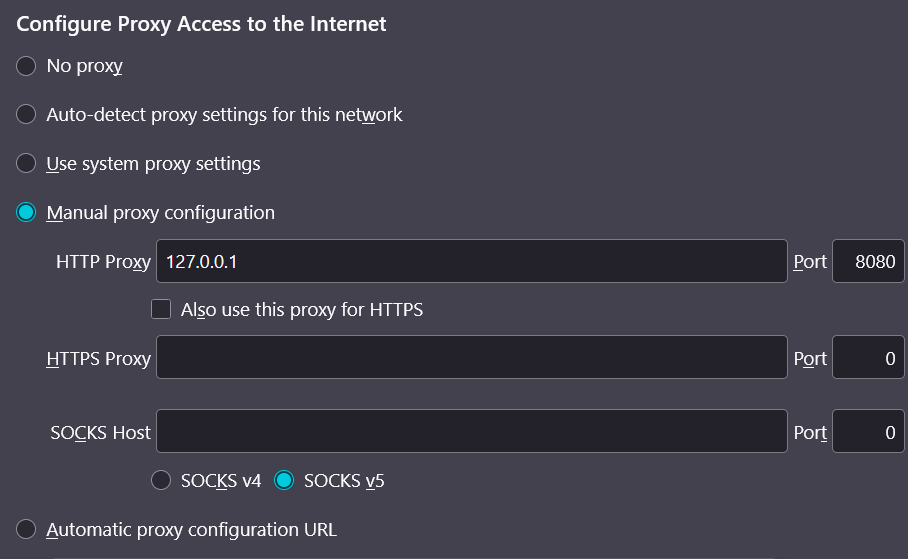
\includegraphics[width=0.8\linewidth]{screenshot002}
		\caption{The browser connection configuration}
		\label{fig:screenshot002}
	\end{figure}
	
	After setting up the browser I compiled my python code and the application started. The main window of the app is presented in figure \ref{fig:screenshot003}.
	
	\begin{figure}[!h]
		\centering
		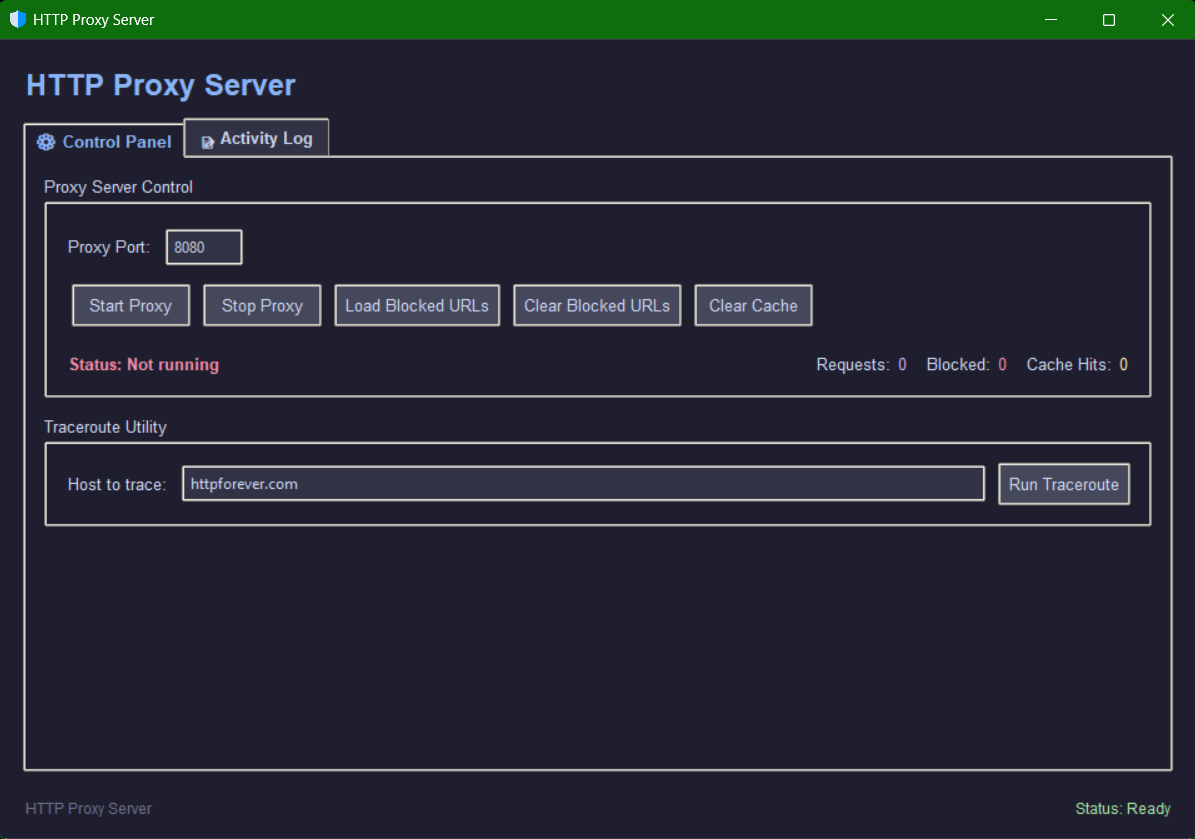
\includegraphics[width=0.8\linewidth]{screenshot003}
		\caption{The main window the proxy app}
		\label{fig:screenshot003}
	\end{figure}
	
	Now I hit the Start Proxy button to start the proxy. The picture of the window after pressing start is demonstrated in figure  in the next page. Notice that the status label changed from a red \textbf{Not running} into a green \textbf{Running on port 8080}.
	
	Lets try to access an http website with and without the proxy server turned on. I used the website \href{http://httpforever.com/}{httpforever} to check the functioning of my proxy.
	
	\pagebreak
	
	\begin{figure}[!h]
		\centering
		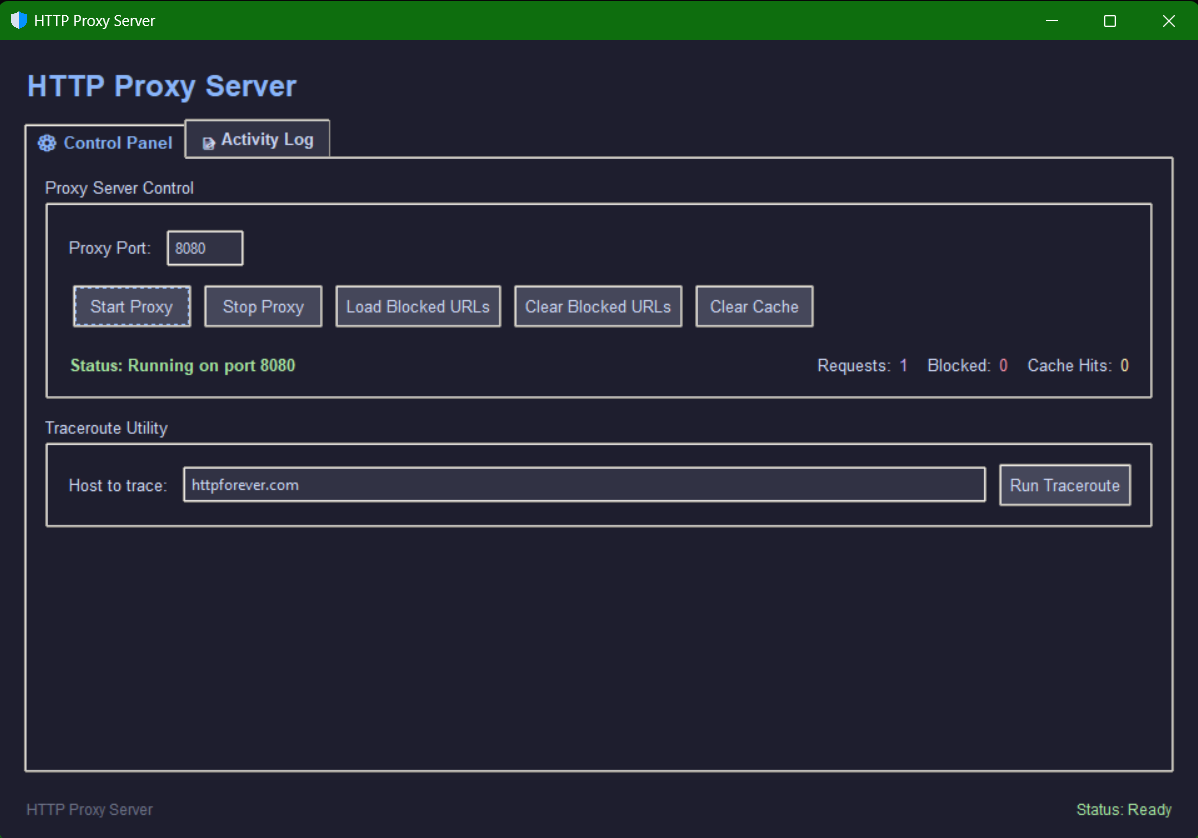
\includegraphics[width=0.8\linewidth]{screenshot004}
		\caption{The main window after hitting start}
		\label{fig:screenshot004}
	\end{figure}
	
	You can see the results below. As expected the website is accessed using the proxy server and denied when the proxy is disconnected.
	
	\begin{figure}[!htb]
		\begin{minipage}{0.49\textwidth}
			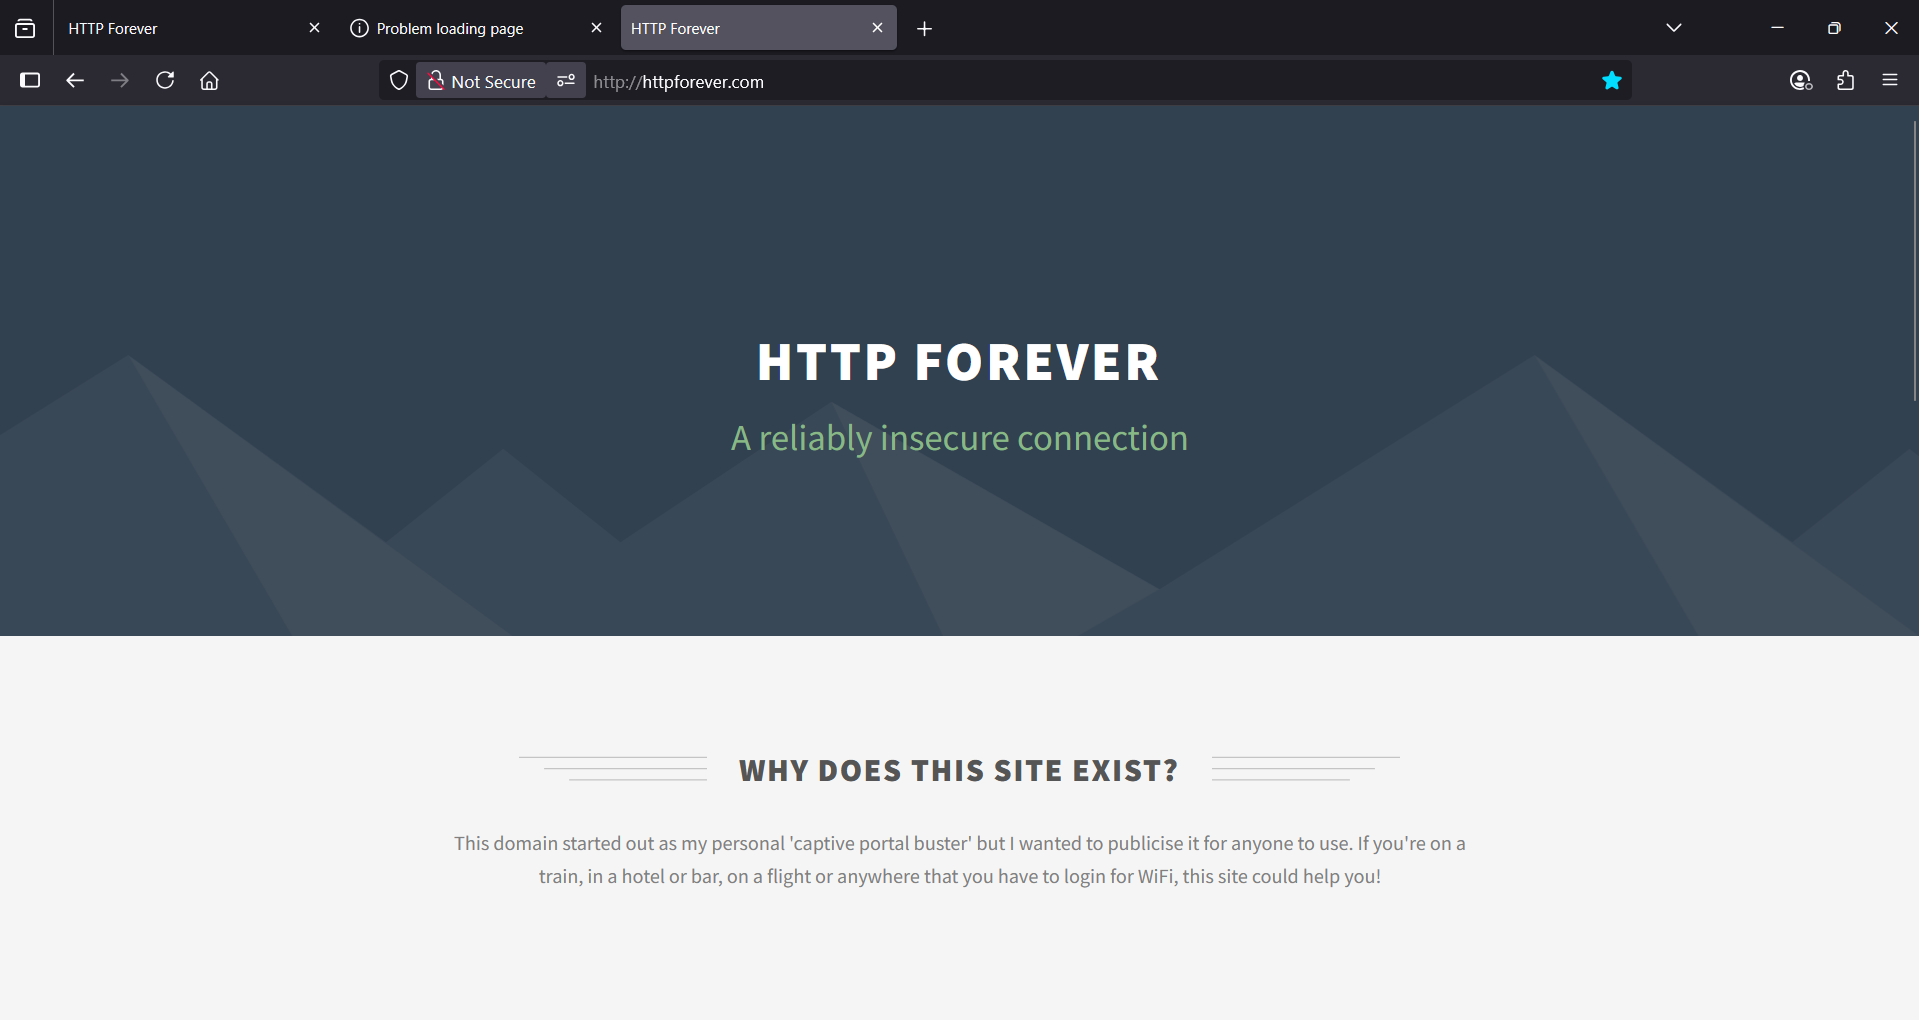
\includegraphics[width=\linewidth]{screenshot006}
			\caption{Proxy Connected}
		\end{minipage}\hfill
		\begin{minipage}{0.49\textwidth}
			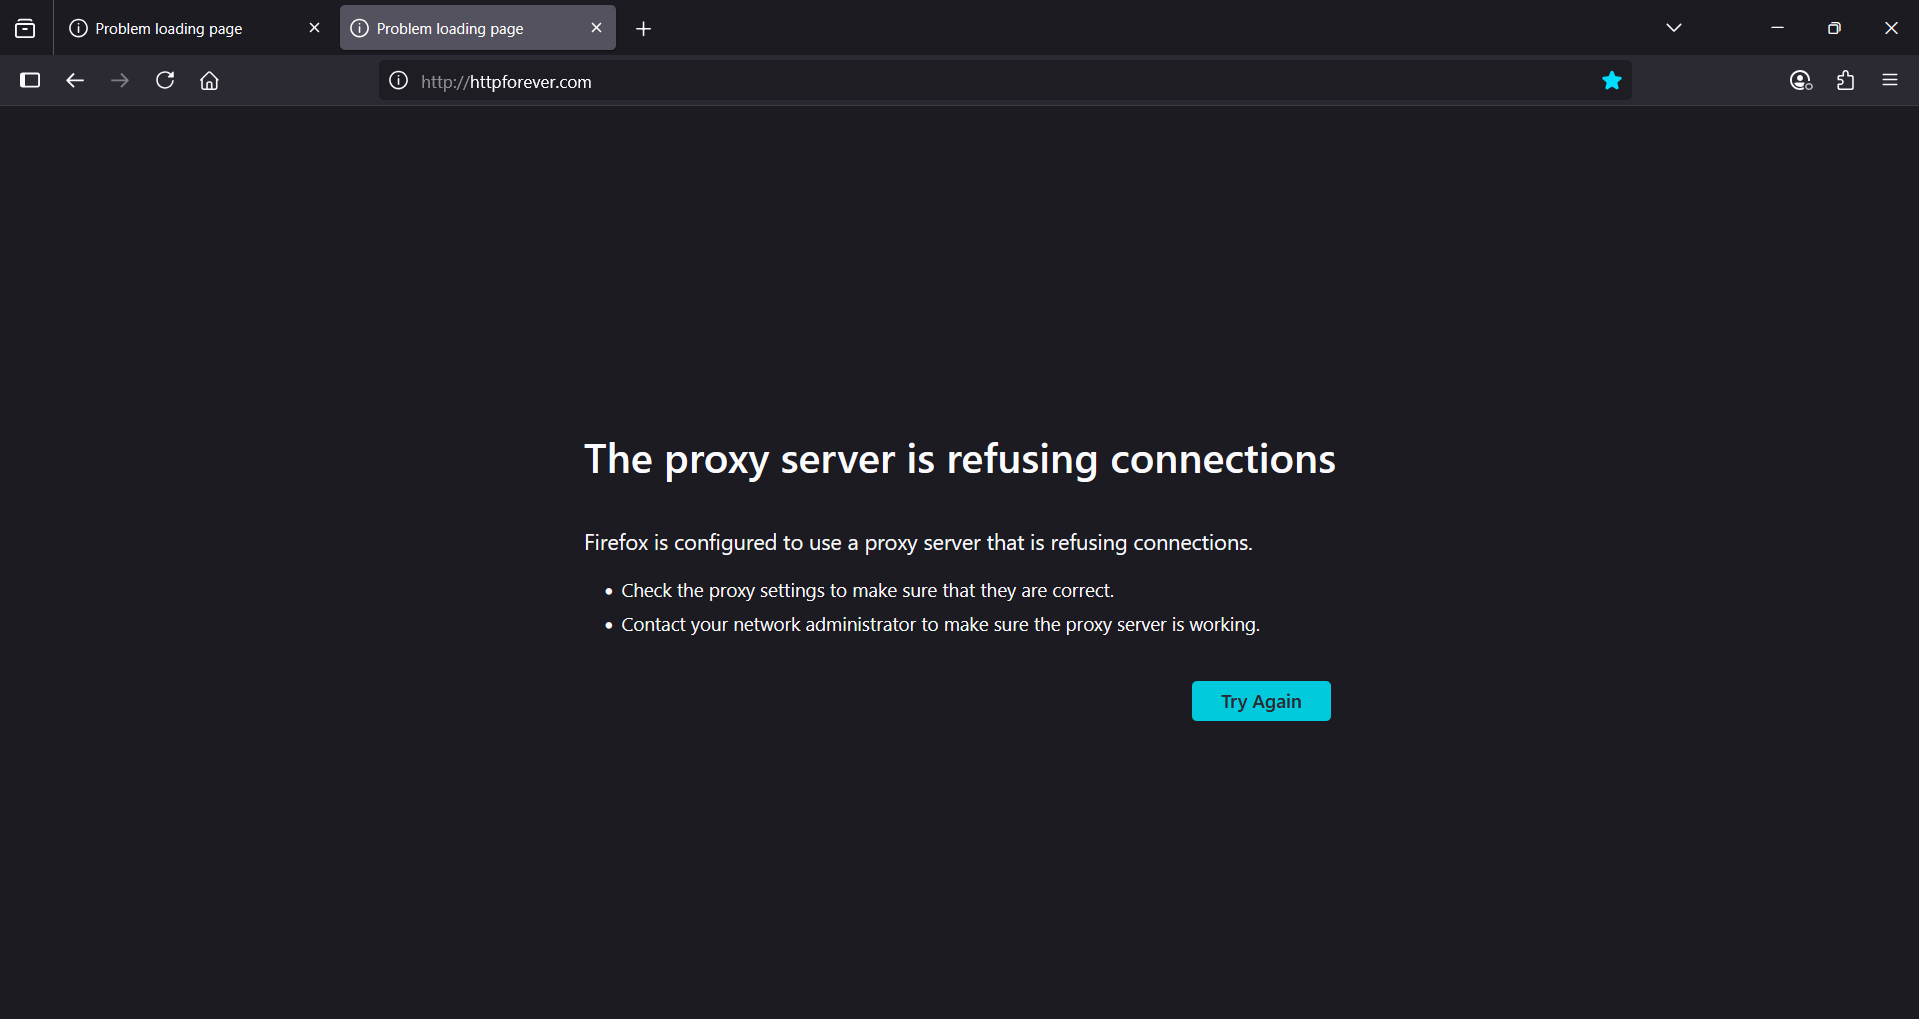
\includegraphics[width=\linewidth]{screenshot005}
			\caption{Proxy Disconnected}
		\end{minipage}\hfill
		\label{1}
	\end{figure}
	
	Lets try the scenario that the port number is less than 1024. I set the port number to 808 and pressed the start button.
	
	It is observed that an error message pops up mentioning that the port number is not valid and the value must be greater than 1024. You can see this result in the figure in the beginning of the next page.
	
	\subsection{URL Blocking}
	There is a text file provided to import as the list of the blocking urls named blocked\_urls. I hit the Load Blocked URLs button and then selected the mentioned file. Then a pop-up appears saying "Loaded 10 blocked URLs" with the title success. Now to see if this really works and the urls in the text file are blocked correctly I accessed \href{http://httpforever.com/}{httpforever} again. I got a \textbf{403 Forbidden} text as a result which is exactly the result we were expecting. You can see the screenshots demonstrating this process in figures \ref{fig:screenshot008}, \ref{fig:screenshot009} and \ref{fig:screenshot010}.
	
	The activity log tab and the event logs after each operation are all displayed in the Log section \ref{sec.log}.
	
	\pagebreak
	
	\begin{figure}[!h]
		\centering
		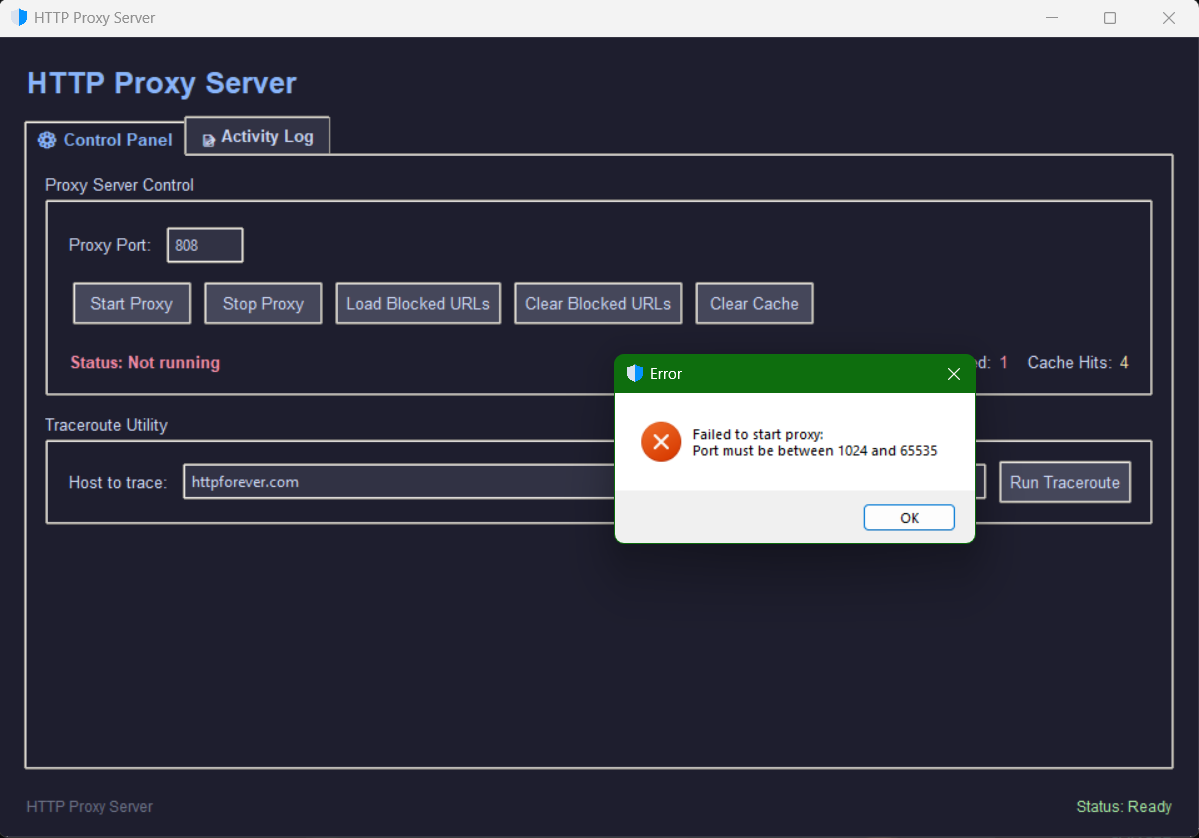
\includegraphics[width=0.62\linewidth]{screenshot007}
		\caption{Port number less than 1024}
		\label{fig:screenshot007}
	\end{figure}
	
	Now to test the correct operation of the Clear Blocked URLs function, I accessed the website again after clicking on the Clear Blocked URLs button. As it was expected, the website loaded properly and without any trouble because the url got out of the black list. It is worth noting that after clicking the button a message showed up telling me that the Blocked URLs cleared!
	
	\begin{figure}[!htb]
		\begin{minipage}{0.49\textwidth}
			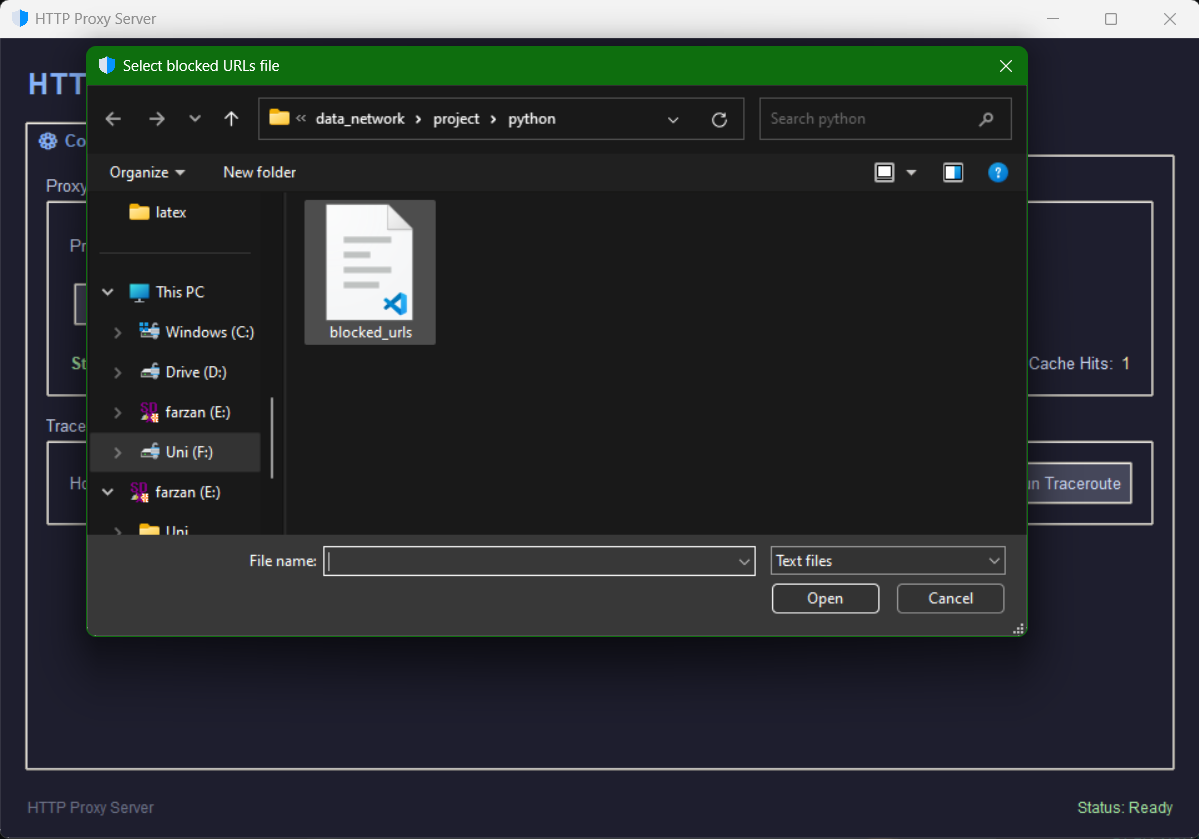
\includegraphics[width=\linewidth]{screenshot008}
			\caption{Selecting the text file containing the list of blocked urls}
			\label{fig:screenshot008}
		\end{minipage}\hfill
		\begin{minipage}{0.49\textwidth}
			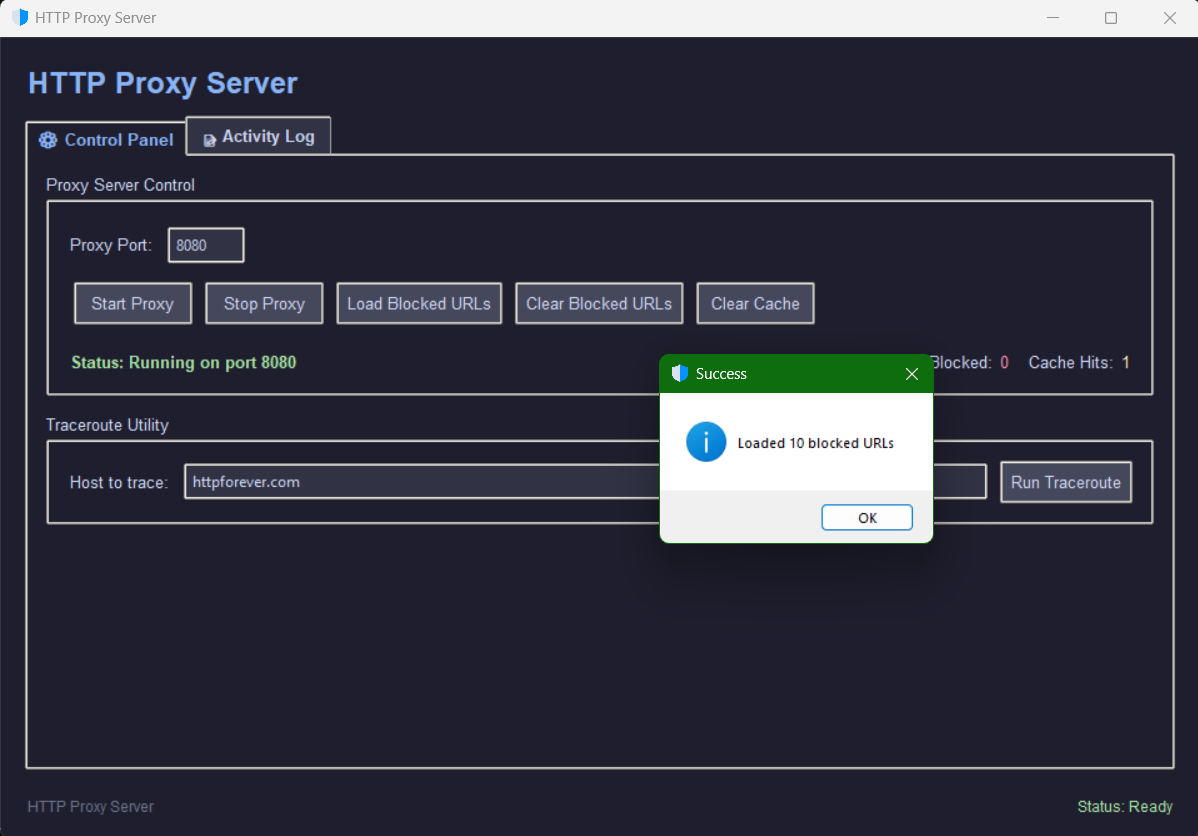
\includegraphics[width=\linewidth]{screenshot009}
			\caption{The pop-up showing that the blocked urls were loaded successfully}
			\label{fig:screenshot009}
		\end{minipage}\hfill
	\end{figure}
	
	\begin{figure}[!h]
		\centering
		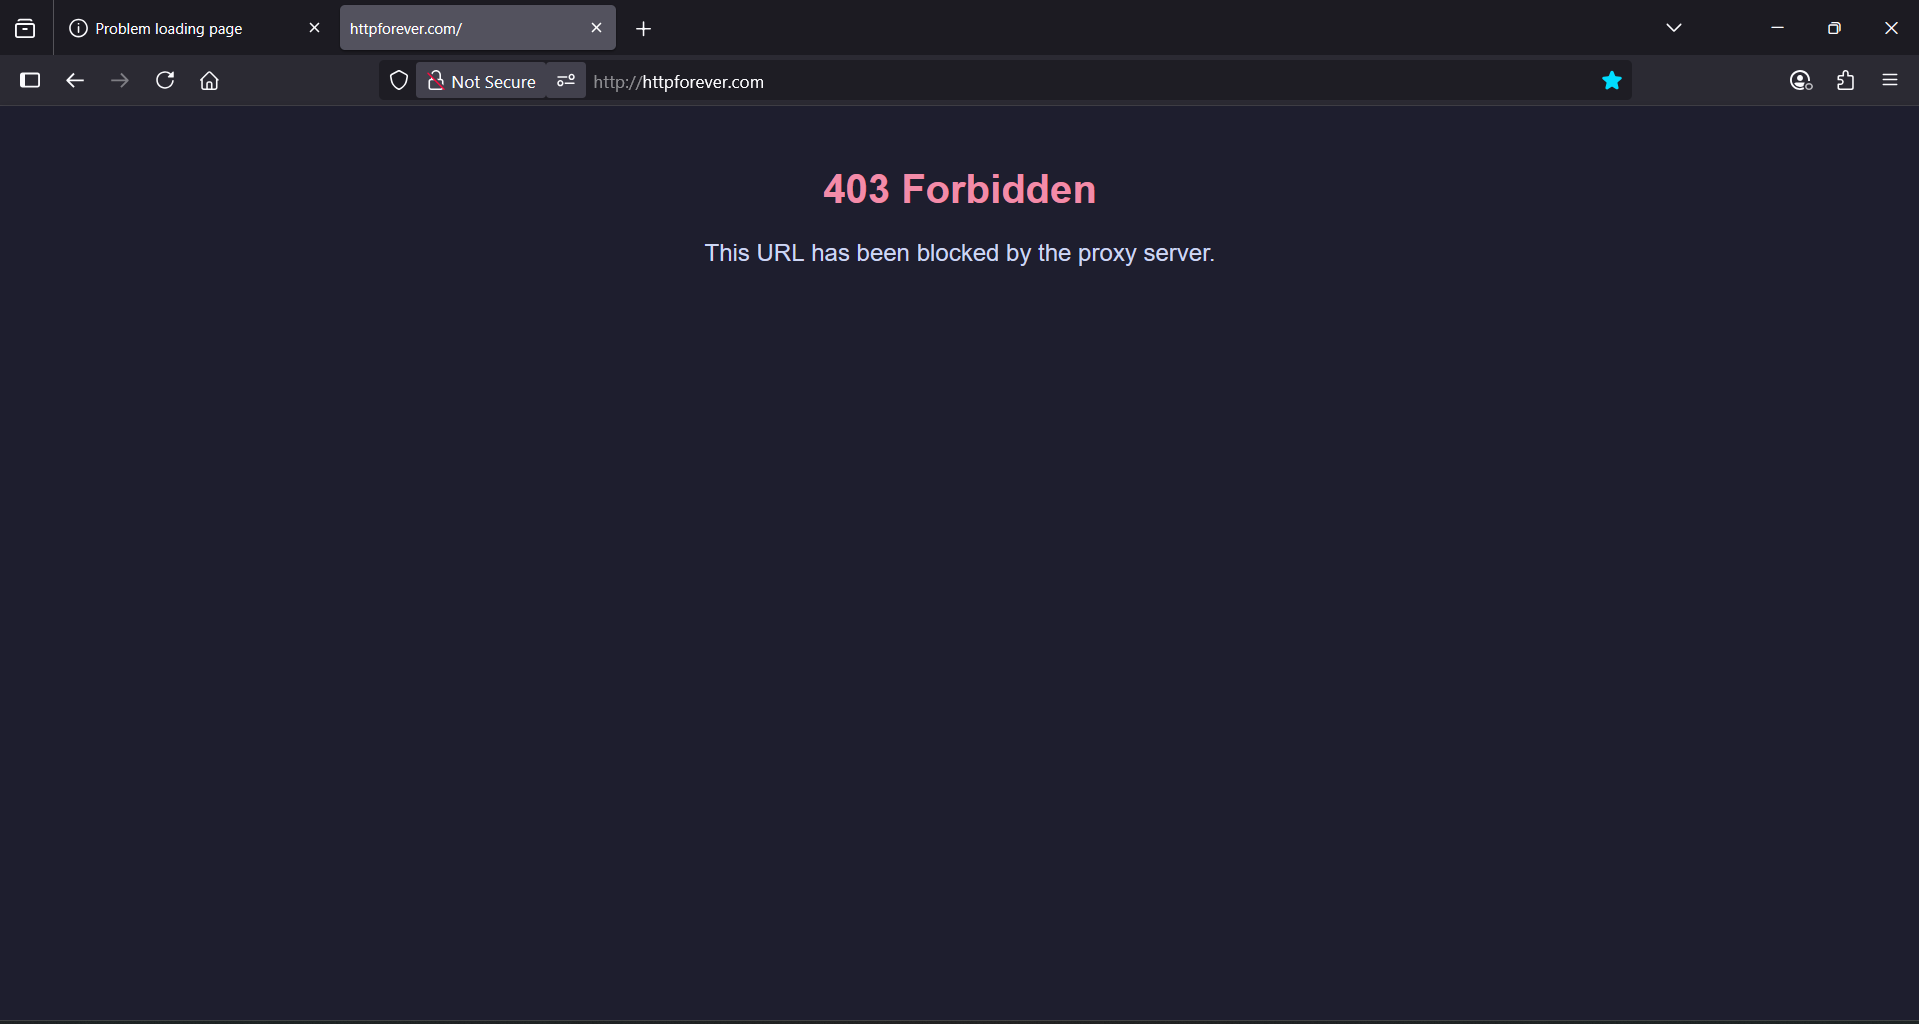
\includegraphics[width=0.65\linewidth]{screenshot010}
		\caption{The result of accessing a blocked url in the browser}
		\label{fig:screenshot010}
	\end{figure}
	
	\pagebreak
	
	\subsection{Caching}
	Now we get to the caching functionality of the proxy server. Each accepted and valid request is saved in the cache storage eventually. After the first attempt to access a website the response gets cached and in the next access attempts the response is send faster because it is forwarded from the cache storage. To test this property I first accessed the test website and then refreshed the page. The content of the page loaded quicker than the first time because the response was saved in the proxy's cache storage and was given to the client immediately.
	
	Then we need to check the Clear Cache button and see if it is functioning accurately. I hit the button and got a "Cache cleared!" message in an info box. Then I accessed the site again and since the cache storage was empty and the saved response was removed, the content of the web page took a little bit longer to load.
	
	\begin{figure}[!h]
		\centering
		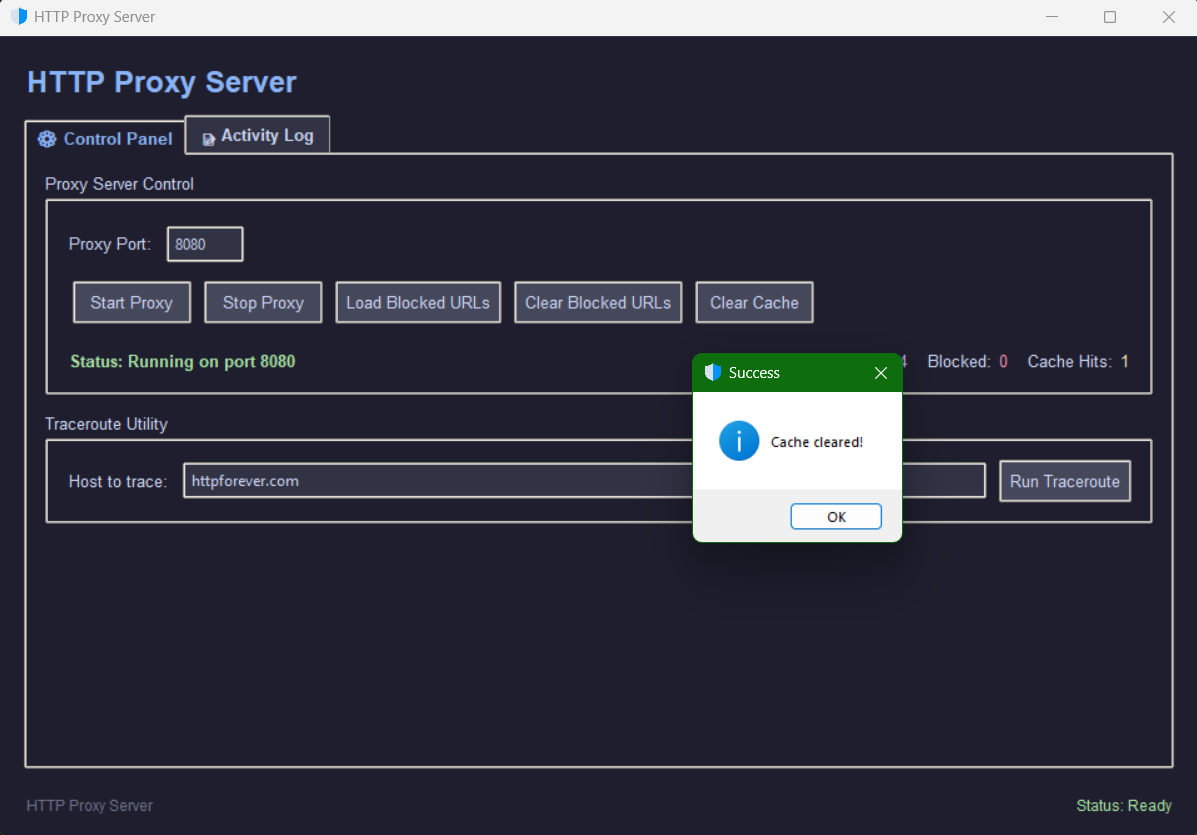
\includegraphics[width=0.62\linewidth]{screenshot011}
		\caption{The Cache cleared pop-up message}
		\label{fig:screenshot011}
	\end{figure}
	
	\subsection{Traceroute}
	It is time to test the interesting option of our proxy app. The traceroute command. The default value in the host url box is the address (url) of the website we used to test our proxy app's capabilities and functions (\href{http://httpforever.com/}{httpforever}). I pressed the run button and waited for a few seconds for the process to finish. Again like the other parts a pop-up message showed up telling me that the traceroute process is completed and I can observe the results in the Activity Log tab.
	
	\begin{figure}[!h]
		\centering
		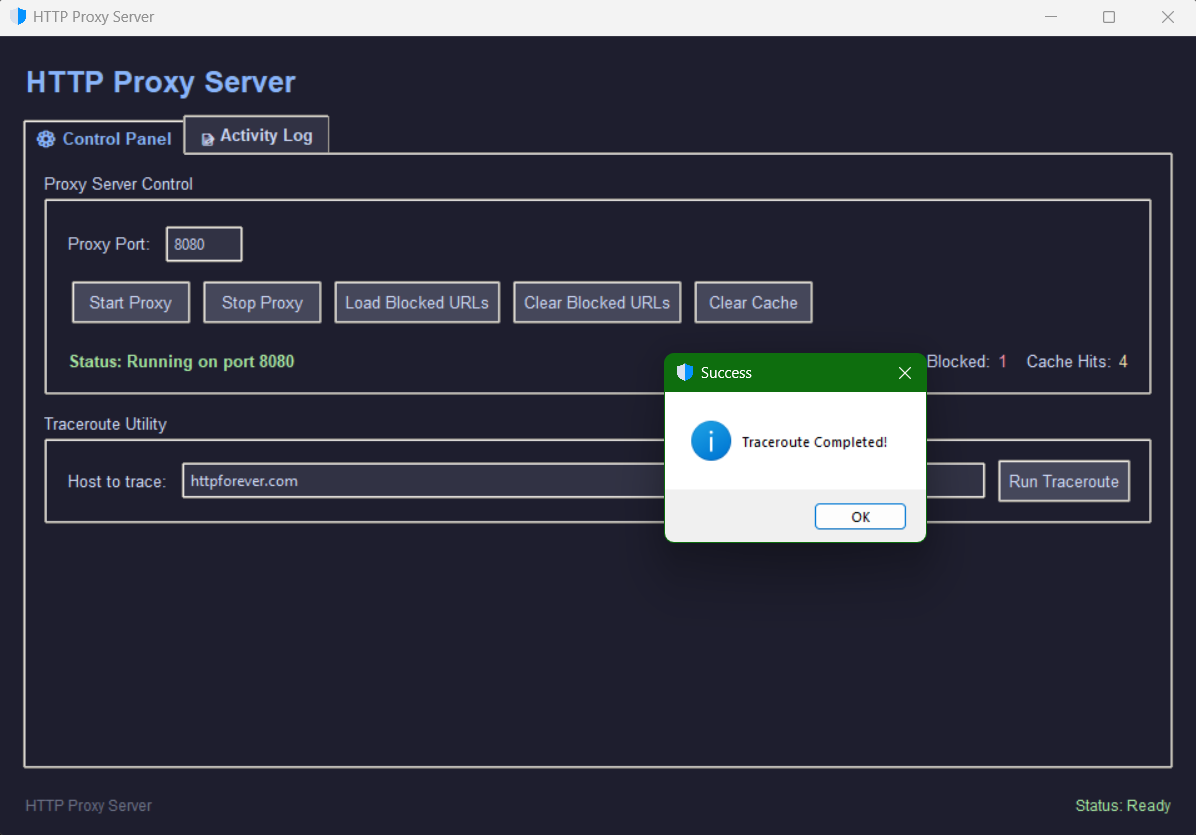
\includegraphics[width=0.62\linewidth]{screenshot012}
		\caption{The Traceroute Completed pop-up message}
		\label{fig:screenshot012}
	\end{figure}
	
	\pagebreak
	
	\subsection{Log}
	\label{sec.log}
	In this section we observe the log messages in the Activity Log tab that appear when something happens. It can be seen in the following figures the screenshots of the activity log before and after the mentioned functions.
	
	\begin{figure}[!htb]
		\begin{minipage}{0.49\textwidth}
			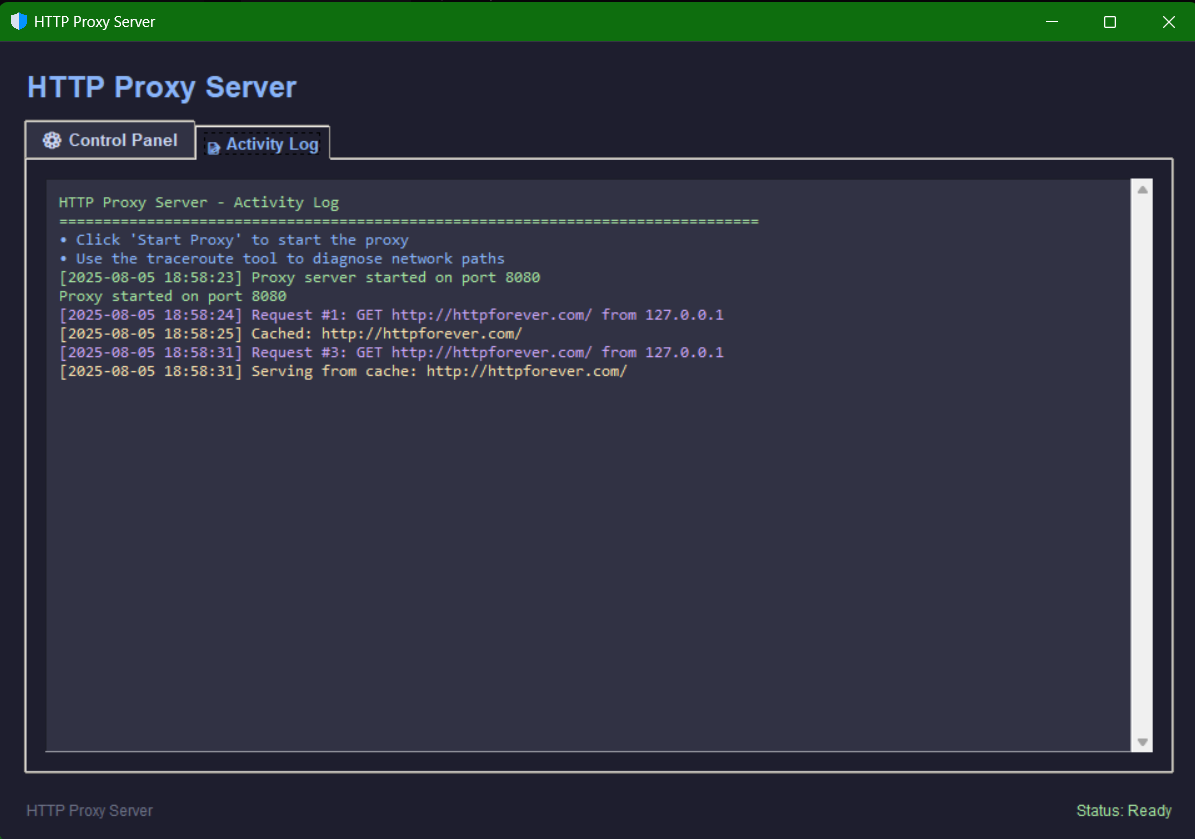
\includegraphics[width=\linewidth]{screenshot013}
			\caption{Access request to the test site, caching process and the result of  access to a cached requests}
			\label{fig:screenshot008}
		\end{minipage}\hfill
		\begin{minipage}{0.49\textwidth}
			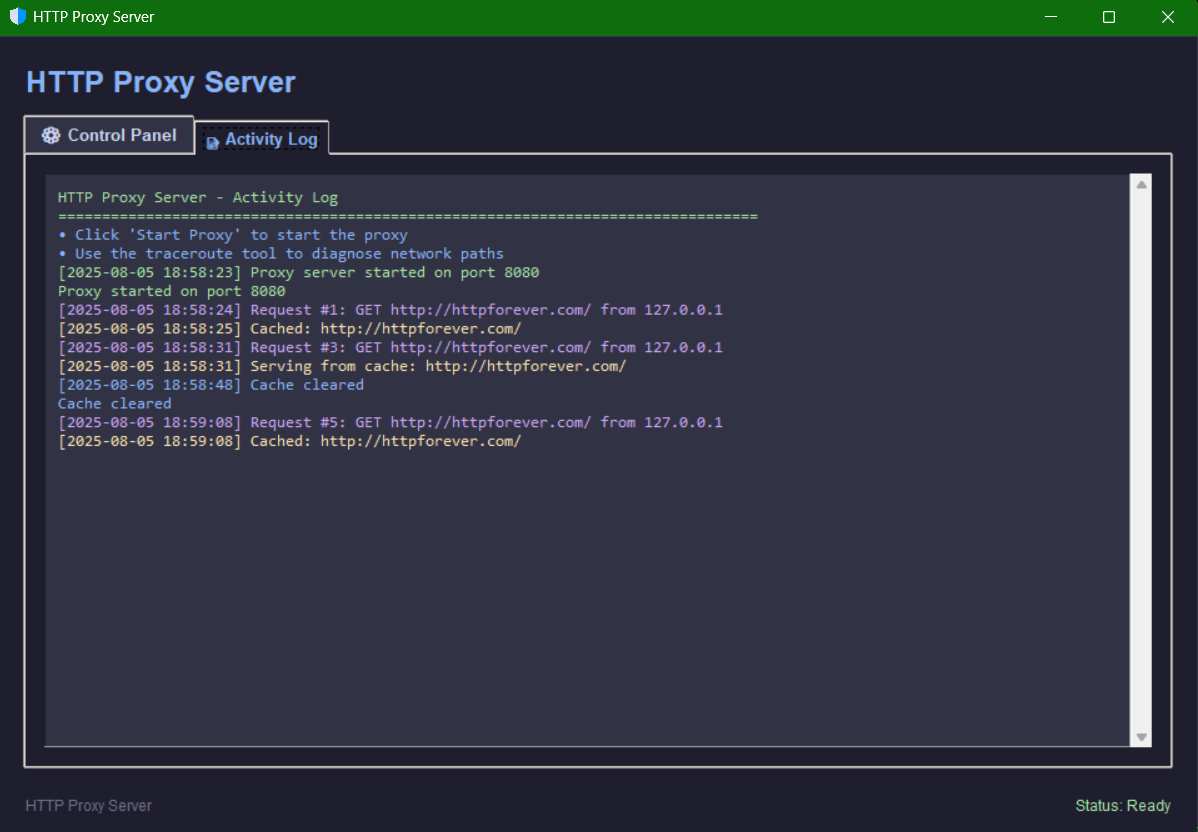
\includegraphics[width=\linewidth]{screenshot014}
			\caption{Clear cache operation message log and the correct operation of the function}
			\label{fig:screenshot009}
		\end{minipage}\hfill
	\end{figure}
	
	\begin{figure}[!htb]
		\begin{minipage}{0.49\textwidth}
			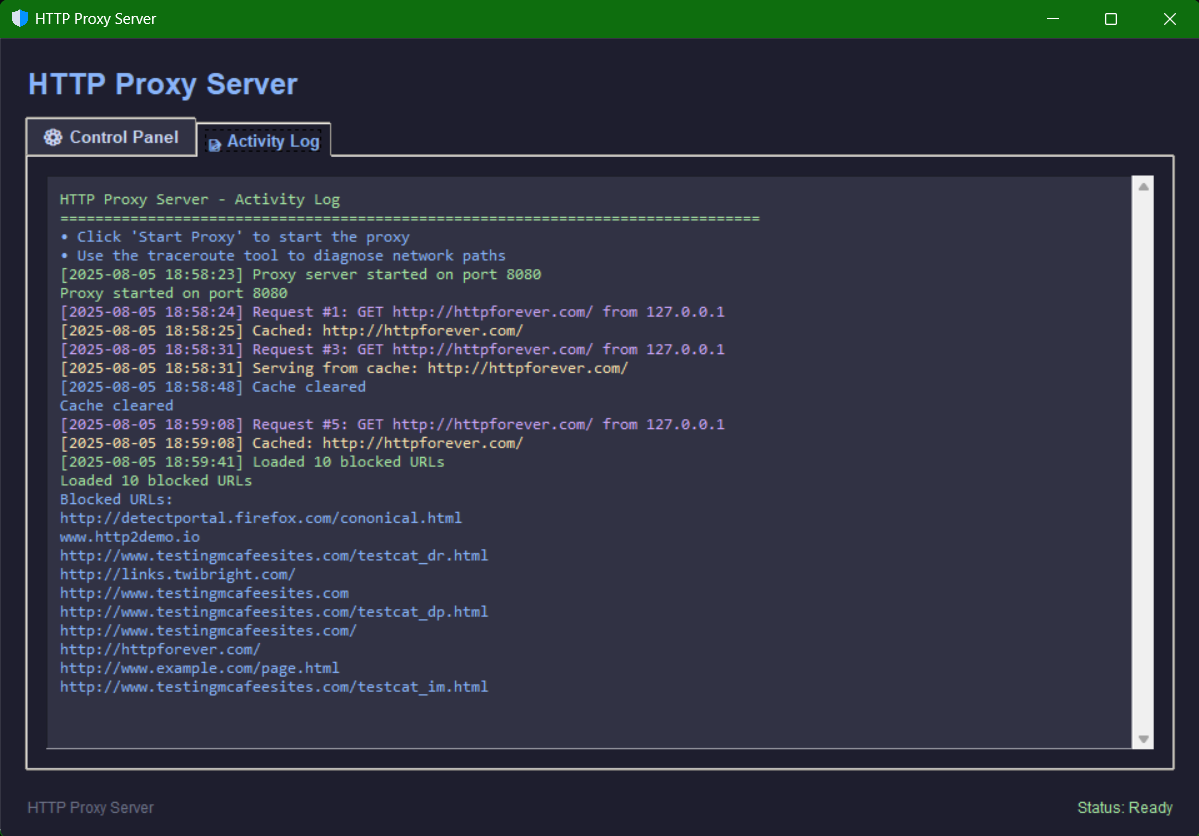
\includegraphics[width=\linewidth]{screenshot015}
			\caption{Load Blocked URLs function result and the list of the blocked urls in the loaded file}
			\label{fig:screenshot008}
		\end{minipage}\hfill
		\begin{minipage}{0.49\textwidth}
			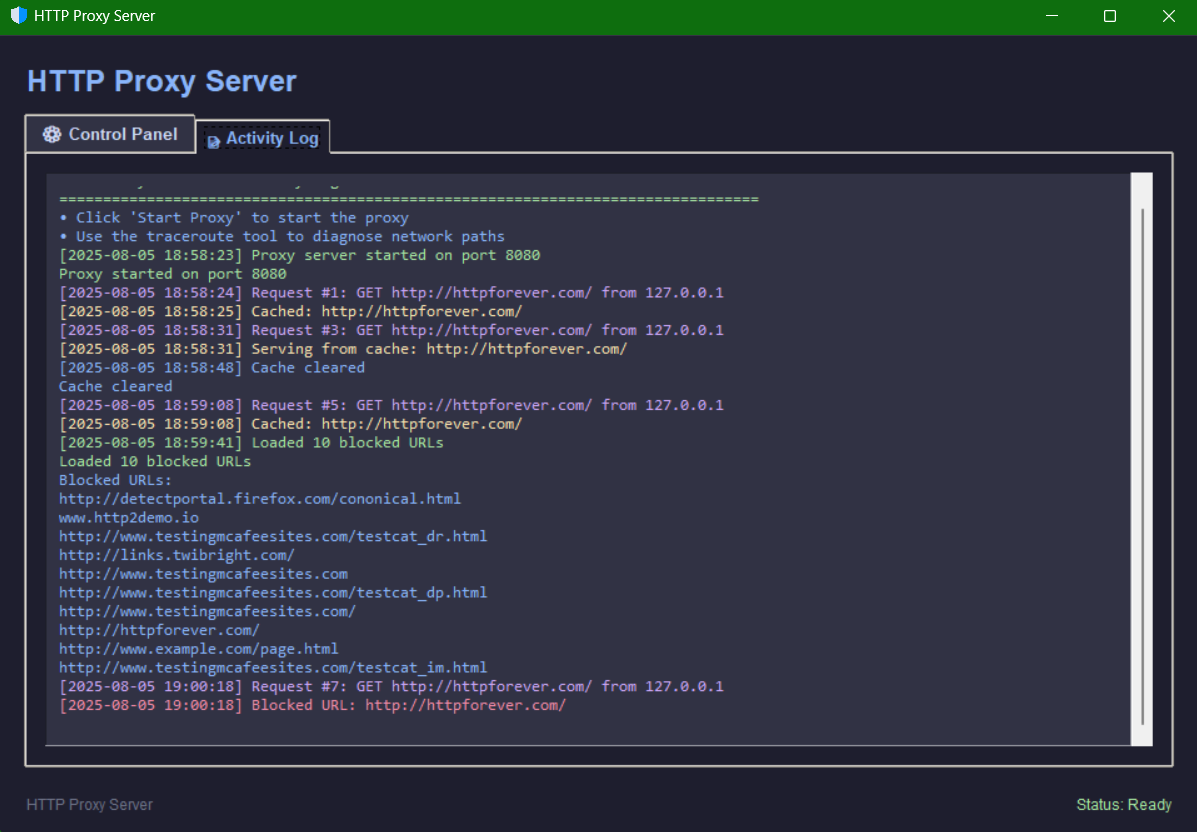
\includegraphics[width=\linewidth]{screenshot016}
			\caption{Requests to blocked urls get blocked by the proxy and a proper message is displayed in the log}
			\label{fig:screenshot009}
		\end{minipage}\hfill
	\end{figure}
	
	\begin{figure}[!htb]
		\begin{minipage}{0.49\textwidth}
			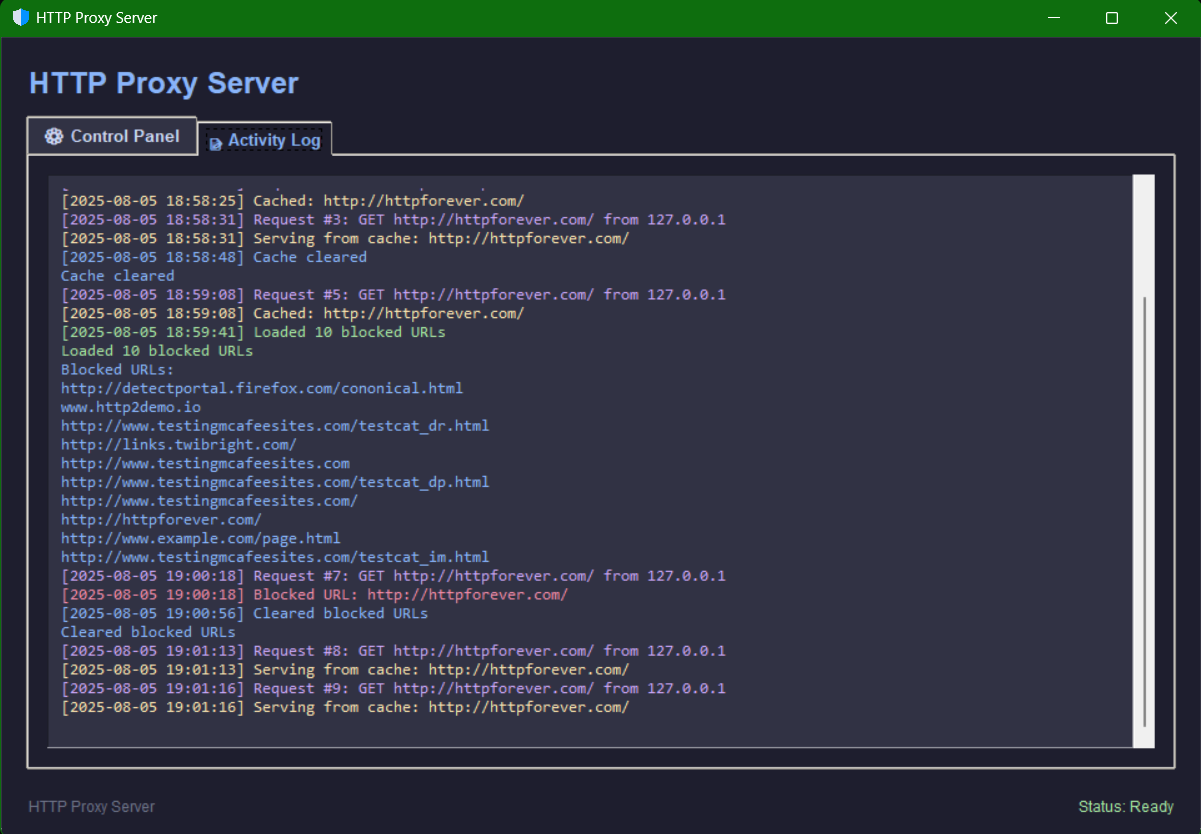
\includegraphics[width=\linewidth]{screenshot017}
			\caption{After deleting the blocked urls list the requests are handled without any problem like before}
			\label{fig:screenshot008}
		\end{minipage}\hfill
		\begin{minipage}{0.49\textwidth}
			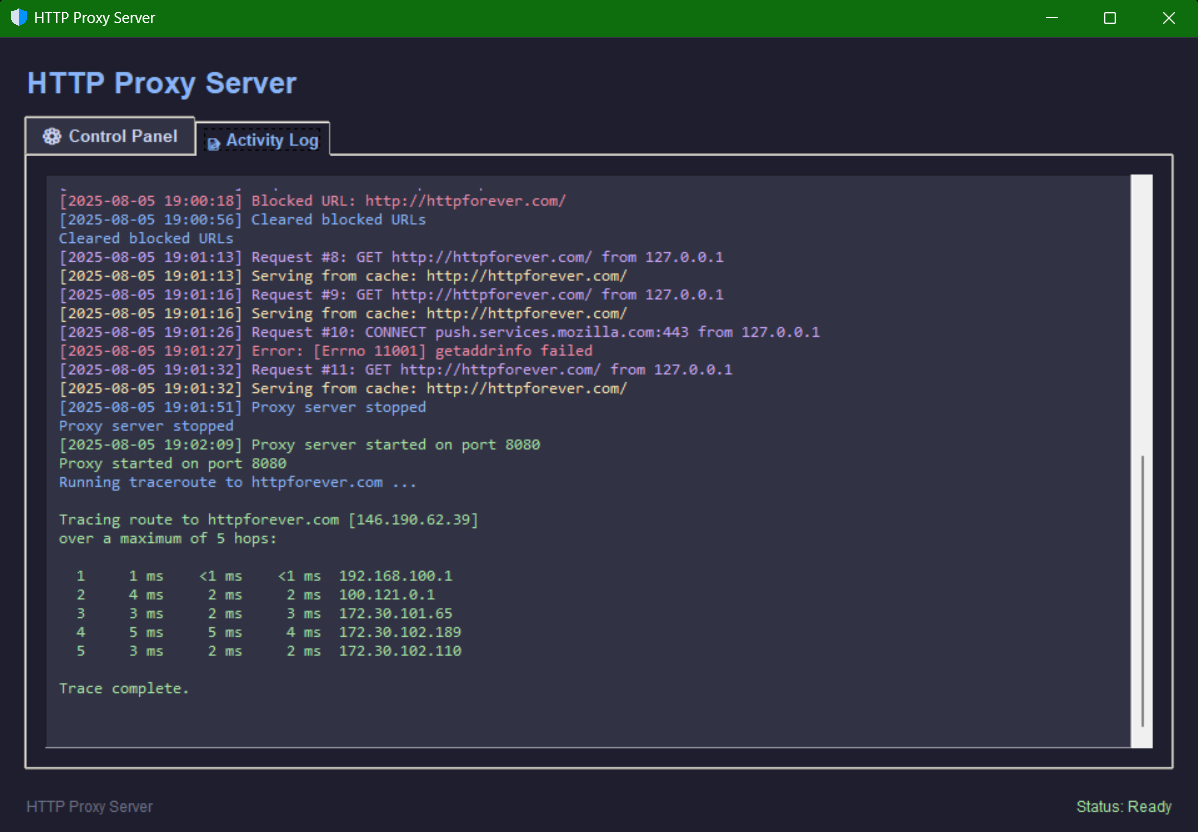
\includegraphics[width=\linewidth]{screenshot018}
			\caption{You can see the results from the traceroute process in the activity log}
			\label{fig:screenshot009}
		\end{minipage}\hfill
	\end{figure}
	
\end{document}